\chapter{Analysis of the Pyramid Wavefront Sensor Signals}\label{CH3}
%Babcock. Summary of some on sky systems. 

A key component of an ExAO system is the wavefront sensor, which measures aberrations from atmospheric turbulence. A common choice of WFS in current and next generation instruments is the pyramid wavefront sensor (PWFS). The PWFS is a highly sensitive wavefront sensor that is able to measure the wavefront at high speeds. The sensitivity and linear range of the PWFS can be tuned by dynamic modulation, making the PWFS robust to different seeing conditions. 

\section{The Pyramid Wavefront Sensor}\label{PWFSintro}
The optical design of the PWFS consists of four components: a focusing optic, the glass pyramid, and a relay lens to image the pupils on the detector \citep{ragazzoni2002pyramid}. Figure \ref{fig:pyramid} shows a schematic of the operation of a PWFS \citep{pyramidfig}.  The starlight is first brought to a focus on the tip of a glass pyramid that splits the focal plane into parts. The apex angle of the pyramid imparts a tilt to separate each of the sections. The result is copies of the telescope pupil that are separated spatially on a detector. The number of pixels across each pupil determines the number of modes the instrument is sensitive to. Current on-sky adaptive optics systems that have a PWFS use a four-sided PWFS. The Magellan Adaptive Optics System (MagAO) \citep{close2018status}, the Large Binocular Telescope Interferometer (LBTI) \citep{esposito2011adaptive}, and MagAO-X use an achromatic double four-sided pyramid. The SCExAO instrument uses two crossed roof prisms as its pyramid optic. The basic PWFS is highly sensitive but suffers from low dynamic range. A modulator is used to move the beam around the pyramid tip to increase the linear range of the PWFS. Modulation is achieved by oscillating a piezo-actuator driven mirror to drive the PSF on the pyramid tip into a circular pattern with a radius quoted in units of $\lambda/D$, where $\lambda$ is wavelength, and $D$ is the diameter of the entrance pupil. This increases the effective spot size on the pyramid tip which increases the sensor's linearity at the cost of sensitivity \citep{guyon2005}.  

\begin{figure}
    \centering
    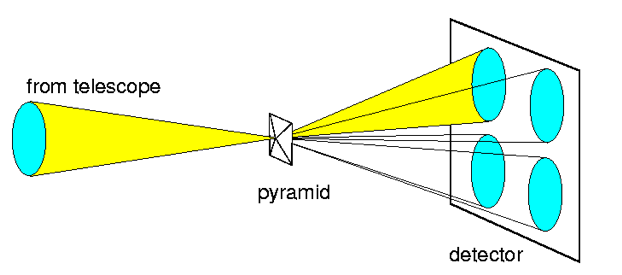
\includegraphics[width=0.75\textwidth]{Chapter Materials/Chapter Two Materials/pyramid.png}
    \caption{Optical design of a PWFS. Light from the telescope is focused onto a glass pyramid tip where it is split and then the pupil plane is reimaged onto a detector. The result is copies of the telescope pupil that contain intensity fluctuations that are related to the wavefront phase.}
    \label{fig:pyramid}
\end{figure}


The intensity measured in the PWFS must be processed to infer the wavefront phase. First, the image is dark subtracted and gain corrected to remove detector artifacts. A threshold mask is then applied to mask out any pixels that do not contain a signal. The wavefront sensor response to a flat wavefront is subtracted off to leave only the intensity pattern caused by the wavefront phase error. The intensity in the pupils can be combined to estimate the wavefront derivative, or slope. We refer to this as the Slopes Maps (SM) calculation. The equation for the 4PWFS is,


\begin{eqnarray}
    S_x=\frac{I_1+I_2-I_3-I_4}{I_1+I_2+I_3+I_4}     \label{4PWFSslopes} \\
    S_y=\frac{I_1-I_2-I_3+I_4}{I_1+I_2+I_3+I_4} \nonumber
\end{eqnarray}

where $S_x, S_y$ are the local wavefront slopes in the x and y direction, and $I_1...I_4$ are the intensity values of the pixel corresponding to the same location in each pupil. The intensity patterns in the pyramid pupils contain both the X and Y spatial information of wavefront gradient from the diffraction off of the pyramid edges. The Raw Intensity (RI) signal processing method uses the pyramid signal as-is. The benefit of the Raw Intensity method is that it is relatively unaffected by alignment errors. The major challenge in using this technique is obtaining a good flat wavefront reference image. The signals in the pyramid pupils are then extracted into a single column vector of intensity values.

All current PWFSs on telescopes use a 4PWFS. ExAO systems need high sampling of the PWFS pupils to optimize performance, and as a result require larger detectors. Detector size, speed, and noise all impose limits on wavefront sensor designs and limit the performance of an GSMT-ExAO system. We are interested in exploring the 3PWFS as an alternative PWFS for an ELT-ExAO wavefront sensor to overcome these limitations. The 3PWFS only has three copies of the pupil and therefore uses fewer detector pixels than the 4PWFS and should be less sensitive to read noise. We assess the performance of the 3PWFS compared to the 4PWFS in simulation to determine if the 3PWFS does outperform the 4PWFS when using high read noise detectors.

To assess the performance of the 3PWFS compared to the 4PWFS, a simulation was developed using the Object Oriented Matlab Adaptive Optics toolkit (OOMAO) \citep{OOMAO}. The OOMAO toolkit is an end-to-end adaptive optics model that can simulate different combinations of guide stars, turbulent atmospheres, wavefront sensors, deformable mirrors, and science cameras. Light is propagated using Fraunhofer diffraction. The PWFS is simulated using a single tip/tilt phase mask that is segmented into N parts. Figure \ref{fig:oomaoFigs}.A and \ref{fig:oomaoFigs}.C show the masks for the 3PWFS and 4PWFS. The masks are scaled and rotated according to a user input for rotation and pyramid apex angle that controls the separation of the pyramid pupils. After scaling, the mask is converted into a phase mask that is applied at the focal plane to simulate a pyramid tip. Figure \ref{fig:oomaoFigs}.C and \ref{fig:oomaoFigs}.D show the resulting pyramid pupils on the simulated wavefront sensor camera, using a flat wavefront and 5 $\lambda/D$ modulation. The master OOMAO toolbox simulates a 4PWFS using Slopes Maps. We extended the PWFS class in OOMAO to include a 3PWFS, taking care that the amplitude of the tip/tilt phase in the 3PWFS phase screen generation matched that of 4PWFS. We included our derivation of the Slopes Maps equation for the 3PWFS (derived in Section~\ref{SlopesDerivation} below), and added the Raw Intensity method for both the 4PWFS and the 3PWFS. For both the Slopes Maps and Raw Intensity method the signal was normalized by the mean value across all valid pixels on the wavefront sensor detector, instead of normalizing pixel by pixel. 

\begin{figure}
    \centering
    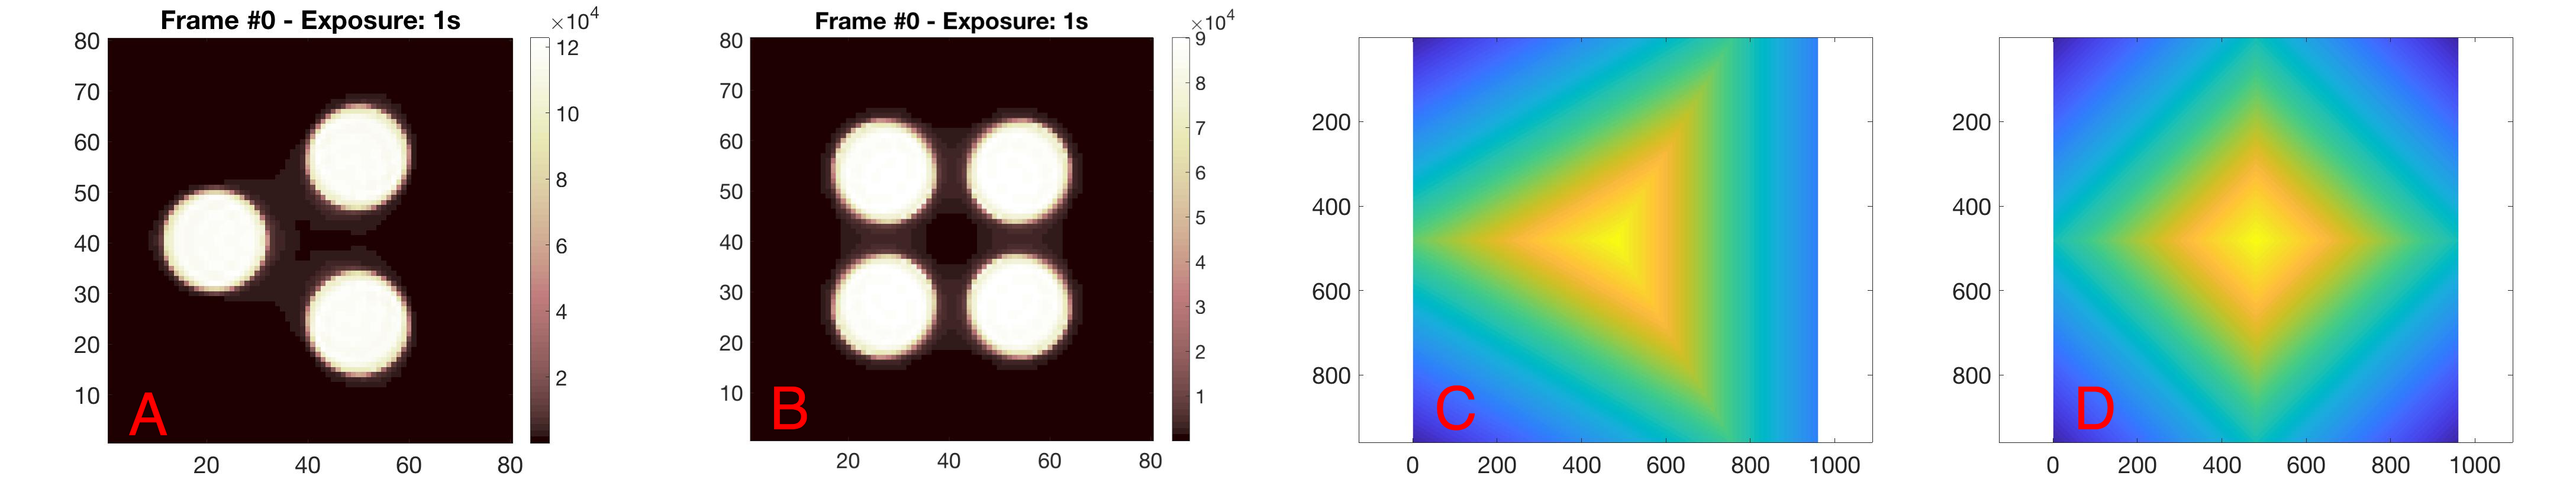
\includegraphics[width=1\textwidth]{Chapter Materials/Chapter Two Materials/oomaoFigs.png}
    \caption{Details of the simulated PWFS in OOMAO. A) and B) The simulated 3PWFS and 4PWFS pyramid masks in OOMAO. These masks are used as a phase screen in the pupil plane to emulate the focal plane splitting and separation done by a real glass pyramid. C) and D) The pupils from the 3PWFS and 4PWFS respectively on the simulated detector. In OOMAO the user can change the size, separation, and intensity values of the pupils through user defined inputs.}
    \label{fig:oomaoFigs}
\end{figure}


\section{Diffraction Theory of the Foucault Test}\label{diffraction}
\subsection{Derivation of Expected Signal from the Foucault Test}
  The PWFS is an extension of the knife edge test: each of the pyramid pupils are the signal from a knife edge test, but include a mirroring effect of the signal across the facets. The underlying physical processes of the pyramid and the knife edge are the same, so we can use the equations that describe the knife edge test explore the operation of the PWFS. The diffraction theory of the PWFS has been studied in detail. \cite{verinaud2004nature} extends the knife edge diffraction theory to model the signal of a roof sensor with dynamic circular modulation. \cite{hutterer2019real} extends the knife edge analysis into general operators such that modulations of any pattern can be modeled. \cite{shatokhina2014fast} presents simplified equations to approximate pyramid signals with and without modulation.\cite{correia2020performance}, and \cite{fauvarque2019kernel} model the pyramid operation as a Fourier filter. In this chapter we use a formalism similar to Vérinaud, but limit our analysis to that of a one dimensional knife edge test for simplicity. We use the knife edge analysis to derive the relationship of the PWFS sensitivity to Fourier modes. Fourier modes have a direct relationship to locations on the focal plane; which is important to coronagraphy because we are trying to maximize the contrast in the dark hole region created by the coronagraph.
 
 In this section we consolidate the diffraction theory of the knife edge test by \citep{linfoot1948theory}, \citep{katzoff1971quantitative}, and \citep{wilson1975wavefront} into a single derivation with uniform notation. Expanding upon their results, we link phase aberrations in the shape of Fourier modes to intensity patterns produced by the knife edge test. We assume a focal plane bisected by a binary amplitude mask representing the knife edge. 
 
 Figure \ref{fig:derivationFlow} describes the steps taken in this derivation. The diagram is in two dimensions for visualization, but in this derivation we assume a one dimensional case for simplicity. We start with an electric field in the entrance pupil, $u_0(x_0)$ that has a phase error given by $\cos(nx)$. A Fourier transform is taken to the focal plane where the knife edge, $H_f(\xi_f)$ is applied. We don't actually solve for $U(\xi_f)$, the electric field in the focal plane, and instead take an inverse Fourier transform to the conjugate pupil plane where the knife edge test signal is found. The electric field at this pupil plane is given by $u(x_i)$, is the convolution of the electric field in the entrance pupil propagated to this pupil plane, $u_0(x_i)$, and the inverse Fourier transform of the knife edge, $h_i(x_i)$. The phase error in the electric field is expanded in a power series, then linearized, and the modulus squared is taken to find the field intensity. By subtracting off the constant term, we are left with the intensity pattern due to only the phase errors. 
 
 
 
 \begin{figure}
     \centering
     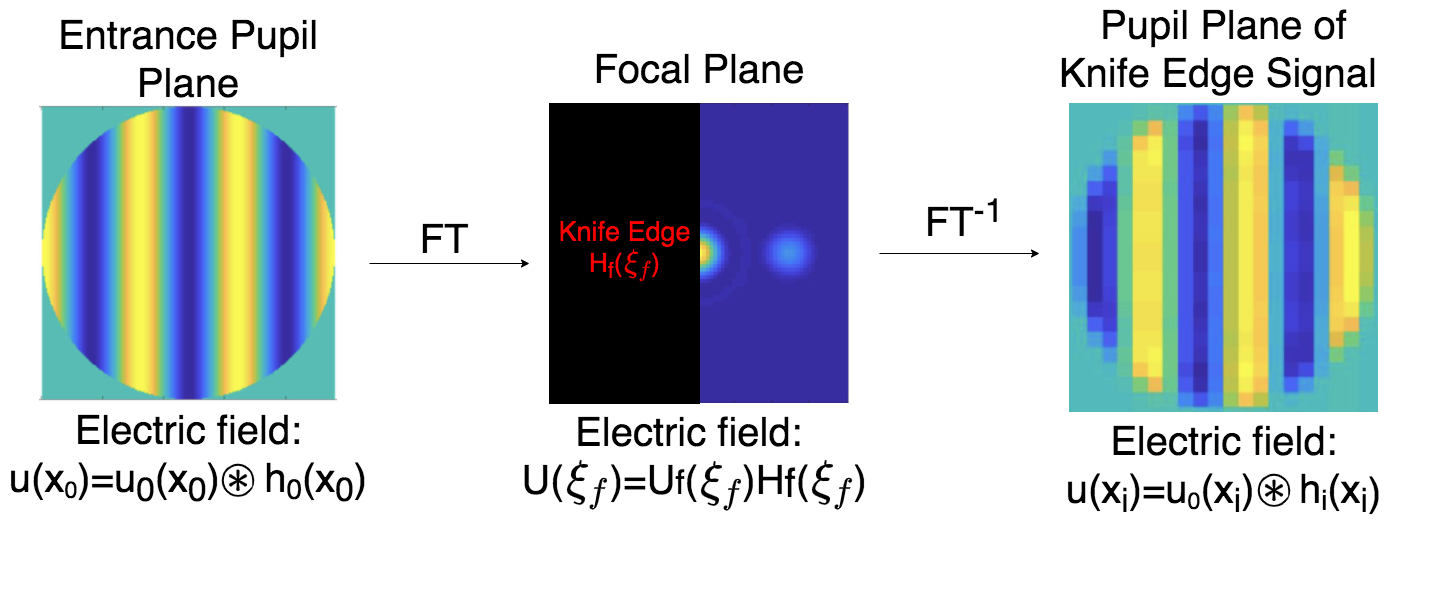
\includegraphics[width=0.9\textwidth]{Chapter Materials/Chapter Two Materials/DerivationFlow.png}
     \caption{Diagram of the steps taken in the derivation. The entrance pupil with electric field $u_0(x_0)$ is Fourier transformed to the focal plane. At the focal plane the knife edge by multiplying the binary mask function of the knife edge, $H_f(\xi_f)$, by the Fourier transform of the electric field in the entrance pupil. An inverse Fourier transform taken to return to the pupil plane where the pyramid signal is detected.}
     \label{fig:derivationFlow}
 \end{figure}
 
 


% To start, we define some terms used in the derivation. 

% \begin{center}
%     \begin{tabular}{ | l |p{12cm}|}
%     \hline
%     $u_0(x_0)$ & Complex wavefront at the "phase object". This could be the surface of a mirror under testing, but for our application it is the phase errors in the pupil caused by atmospheric turbulence. \\ \hline
%     $u_i(x_i)$ & Complex wavefront at the image plane. For the pyrmaid wavefront sensor the image plane is the pupil plane. \\ \hline
%     $h(x_i)$ & The impulse response of the system. \\ \hline
%     $m(x)$ & The equation of phase error to be measured. $u(x)=exp(-2\pi i m(x))$  \\ \hline
%     $p(x_i )$ & The intensity pattern at the image plane due to the diffraction of the electric field with the knife-edge \\ \hline
%     \end{tabular}
% \end{center}

To start we define the electric field in the entrance pupil as $u_0(x_0)$. We take the Fourier transform the of the electric field to get to the focal plane, where we will apply the knife-edge. The Fourier transform is here defined as,

\begin{equation}
    \mathcal{F}\{\xi_x\}=\frac{1}{2\pi}\int_{-\infty}^\infty e^{-i x \xi_x} f(x) dx
    \label{FourierT}
\end{equation}

\noindent where $\xi_x$ is the spatial frequency corresponding to the spatial coordinate $x$. $\mathcal{F}\{\cdot\}$ denotes the Fourier transform operator, and  $\mathcal{F}^{-1}\{\cdot\}$ will denote its inverse. The equation of the electric field in the focal plane, $U(\xi_f)$ is:

\begin{equation}
    U (\xi_f)=U_f(\xi_f)H_f(\xi_f)
    \label{FT}
\end{equation}

\noindent where,
% We now multiply the transmission function of the knife edge, $H(\xi_x)$. In this derivation we assume that the knife edge is like a step function, the transmission of light is 1 until the edge of the knife edge is reached and then drops to zero. We assume for simplicity that the aperture is infinite, but that the knife edge eclipses half of it. After multiplication, the Fourier transform of equation must be taken again to calculate the electric field in the pupil plane. We write out the step function in terms of the sign function $sgn(\xi_x)$, in order to calculate the Fourier Transform easily. The transfer function of the knife edge is given by the following equation.
\[ 
H_f(\xi_f)= 1/2+1/2\mbox{sgn}(\xi_f) \left\{
\begin{array}{ll}
      1 \: for \: \xi_f >0\\
      0 \: for \: \xi_f <0\\
      
\end{array} 
\right. 
\]

\noindent is the binary mask function of the knife edge, and $U_f(\xi_f)$ is the Fourier transform of $u_0(x_0)$. Taking the inverse Fourier transform brings us to the conjugate pupil plane. The inverse Fourier transform of $H_f(\xi_f)$ is

% \begin{equation}
%      FT^{-1}[H(\xi_x)]=\frac{1}{2\pi}\int_{-\infty}^\infty e^{ i x \xi_x} ( \frac{1}{2}+\frac{1}{2}sgn(\xi_x)) d\xi_x \\
%  =\frac{1}{2}\delta(-x)+\frac{i}{2\pi}(\frac{1}{x})
% \label{delta}
% \end{equation}

\begin{equation}
    h_i(x_i)= \mathcal{F}^{-1}[H_f(\xi_f)] =
    % \frac{1}{2\pi} \int_{-\infty}^\infty e^{ i x \xi_f}
    % \left(
    %     \frac{1}{2} + \frac{1}{2} \mathrm{sgn}(\xi_f)
    % \right) d\xi_f
    % = 
    \frac{1}{2} \delta(-x_i) + \frac{i}{2\pi} \left(\frac{1}{x_i}\right)
\label{delta}
\end{equation}


%  = \frac{1}{2} \frac{1}{2\pi} \int_{-\infty}^\infty e^{- i x \xi_x}d\xi_x+\frac{1}{2} \frac{1}{2\pi}\int_{-\infty}^\infty e^{- i x \xi_x}sgn(\xi_x) d\xi_x
% \end{align*}

% We make use of the property of the delta function to solve for the Fourier Transform of $\frac{1}{2}$:

% \begin{equation}
%     \delta(x)=\frac{1}{2\pi}\int_{-\infty}^\infty e^{ i x \xi_x}d\xi_x
% \end{equation}

% which leads to,
    
% \begin{equation}
%     \frac{1}{2}\delta(x)=\frac{1}{2}\frac{1}{2\pi}\int_{-\infty}^\infty e^{ i x \xi_x}d\xi_x 
% \end{equation}

% where $\frac{1}{2}\delta(x)$ is the Fourier Transform of $\frac{1}{2}$. To solve for the Fourier transform of $\frac{1}{2} sgn(\xi_x)$ function, we use the derivative property.

% \begin{equation}
%   FT[\frac{d g(x)}{dx}]=i2\pi \xi_x G(\xi_x)
%   \label{derivativeProp}
% \end{equation}

% where the derivative of $\frac{1}{2} sgn(\xi_x)$ is $\delta(\xi_x)$. Plugging this into Equation~\ref{derivativeProp}, gives the result,
% \begin{equation}
%   FT[\frac{d sgn(\xi_x)}{d\xi_x}]=FT[\delta{\xi_x}]=1=2\pi i x G(x).
% \end{equation}

% Solving for $G(x)$,
% \begin{equation}
%  G(x)=\frac{1}{i2\pi x}.
% \end{equation}

% Now we can sum our answers to get the Fourier Transform of a step function.

% \begin{equation}
%  FT[step(\xi_x)]=\frac{1}{i2\pi x_i}+\frac{1}{2}\delta(x_i)
%  \label{knifeedge}
% \end{equation}

We take the results of Equation~\ref{delta} and convolve it with $u_0(x_i)$, which is the Fourier transform of $U_f(\xi_f)$ in Equation~\ref{FT}, to get the electric field at the pupil plane, $u(x_i)$. The resulting equation is Equation 5a from Wilson.\citep{wilson1975wavefront}


% \begin{equation}
%   u_i(x_i)= u_0(x_0) \circledast \frac{i}{2\pi x_i}+\frac{1}{2}\delta(-x_i) 
%  = \int_{-\infty}^\infty u_0(x')[\frac{1}{2}\delta(x'-x_i)+\frac{i}{2\pi}\frac{1}{x_i-x'}]dx' 
% \end{equation}
%  \begin{equation}
%       u_i(x_i) =\frac{1}{2}u_0(x_i)+\frac{i}{2\pi}\int_{-\infty}^\infty \frac{u_0(x')dx'}{x_i-x'}
%       \label{KEconv}
%  \end{equation}

\begin{equation}
    u(x_i)= u_0(x_i) \circledast \left(
        \frac{i}{2\pi x_i}+\frac{1}{2}\delta(-x_i)
    \right)
    =
    \int_{-\infty}^\infty
    u_0(x') \left[
        \frac{1}{2}\delta(x'-x_i)+\frac{i}{2\pi}\frac{1}{x_i-x'}
    \right] dx' 
    \label{KEconv}
\end{equation}

The first modification to Equation~\ref{KEconv} by Wilson and Katzoff is to assume that the pupil has a finite aperture, resulting in the integral limits of -1 to 1. The following equations are equations 6 through 9 in Wilson's paper \citep{wilson1975wavefront}. For a perfect wavefront we assume $u_0 (x_i )=1$.  Wilson and Katzoff define $m(x)$ as the local mirror error in half-wavelengths, but for our application it would be the phase errors caused by atmospheric turbulence. Assuming an electric field with some phase error $m(x)$ we first expand the electric field as a Taylor series as follows,
\begin{equation}
    u_0 (x_i )=e^{(-2\pi i m(x_i ))}=1-2\pi i m(x_i )-2\pi^2*m^2 (x_i )+...
    \label{taylorexp}
\end{equation}
\noindent and disregard all higher order terms. Substituting Equation~\ref{taylorexp} into Equation~\ref{KEconv} and simplifying gives:

% \begin{equation}
%     2\pi*u_i (x_i )=\pi[1-2\pi^2 m^2 (x_i )+2\int_{-1}^1\frac{m(x')}{x'-x_i} dx']
% +i[-2\pi^2 m(x_i)+\int_{-1}^1\frac{dx'}{x'-x_i}-2\pi^2\int_{-1}^1\frac{m^2(x')}{x'-x_i}dx']
% \end{equation}
\begin{multline}
    2\pi u(x_i ) = 
    \pi 
    \left[ 
        1-2\pi^2 m^2 (x_i )+2\int_{-1}^1 \frac{m(x')}{x'-x_i} dx'
    \right] \\
    +   i \left[
        -2\pi^2 m(x_i)+\int_{-1}^1\frac{dx'}{x'-x_i}
        -
        2\pi^2\int_{-1}^1\frac{m^2(x')}{x'-x_i}dx'
    \right]
\end{multline}



The intensity in the image plane is the modulus squared of this expression, of which we keep only the linear terms:

% As a side note the integral:$\int_{-1}^1\frac{dx'}{x'-x_i}$ is equal to $ln(\frac{1-x}{1+x})$.

% \begin{equation}
%     I(x_i)=\pi^2 + \ln^2(\frac{1-x}{1+x})+4\pi^2\int_{-1}^1\frac{m(x')}{x'-x_i} dx'-4\pi^2 m(x_i)\ln(\frac{1-x}{1+x})
% \end{equation}
\begin{equation}
    I(x_i) = \pi^2 + \ln^2 \left(
        \frac{1-x_i}{1+x_i}
    \right)
    +
    4 \pi^2 \int_{-1}^1 \frac{m(x')}{x'-x_i} dx'
    -
    4\pi^2 m(x_i) \ln\left(
        \frac{1-x_i}{1+x_i}
    \right)
\end{equation}

The result contains two constant terms, which represent the intensity response $I_r(x_i )$, which is the reference intensity pattern resulting from a perfect wavefront propagated through the optical system. This can be subtracted out. The other two terms are dependent on the shape of the wavefront error. After subtracting  $I_r (x_i )$ and dividing by $4\pi^2$ we are left with the intensity pattern due to a pure phase error $I_p(x_i)$:

% \begin{equation}
%     p(x_i)=\frac{I(x_i)-I_0(x_i)}{4\pi^2}\int_{-1}^1\frac{m(x')}{x'-x_i} dx'-m(x_i)\ln(\frac{1-x}{1+x}).
% \end{equation}

\begin{equation}
    I_p(x_i) = \left(\frac{I(x_i) - I_r(x_i)}{4\pi^2}\right)=
     PV \int_{-1}^1 \frac{m(x')-m(x_i)}{x'-x_i}dx'
\end{equation}    
    % \int_{-1}^1\frac{m(x')}{x'-x_i} dx'
    % -
    % m(x_i)\int_{-1}^1\frac{dx'}{x'-x_i} 


% Collecting all constant terms into $C$, we can combine the two terms above into a single equation.
% \begin{equation}
%     I_p(x_i)=C \left( PV \int_{-1}^1 \frac{m(x')-m(x_i)}{x'-x_i}dx'\right)
% \end{equation}

In this equation $PV$ stands for the principal value. The $PV$ is used to evaluate integrals that have a discontinuity, in our case this is when $x_i=x'$ \citep{johansson1999hilbert}. This is the result found by \cite{linfoot1948theory}, and is the equation currently used to describe the operation of the PWFS  \citep{verinaud2004nature}. In high contrast imaging we are interested in the effect of phase errors at different spatial frequencies as these correspond to contrast at specific locations in the post-coronagraphic focal plane. \cite{katzoff1971quantitative} showed that this equation accurately predicts the intensity pattern from phase errors that are described by a power series, $x^{N}$, but his solution to the expected intensity pattern due to phase errors in the form of sines and cosines does not match the signal from the PWFS. To find the response of a knife edge to an error of the form $\cos(nx)$, where $n$ is the spatial frequency, we need to modify the above derivation. In this derivation we assume an infinite aperture approximation, and take the integral from $-\infty$ to $\infty$ instead of from -1 to 1. We start at Equation~\ref{taylorexp}, and consider only the linear component and substitute into Equation~\ref{KEconv}.  The electric field at the entrance aperture is now: 


\begin{equation}
    u_0(x_i )=\exp(-2\pi i m(x_i ))=1-2\pi i m(x_i).
    \label{EF}
\end{equation}

We substitute Equation~\ref{EF} into Equation~\ref{KEconv} to find the electric field in the pupil plane $u(x_i)$, which yields:

\begin{equation}
    u(x_i)= \frac{1}{2}(1-2\pi i m(x_i))+\frac{i}{2\pi}\int_{-\infty}^\infty \frac{(1-2\pi i m(x'))dx'}{x_i-x'}
    \label{HT}
\end{equation}

Expanding the integral, we have:
\begin{equation}
    u(x_i)= \frac{1}{2}(1-2\pi i m(x_i))+\frac{i}{2\pi}\int_{-\infty}^\infty \frac{dx'}{x_i-x'}+\int_{-\infty}^\infty \frac{ m(x')dx'}{x_i-x'}
\end{equation}

\noindent where the integrals are now in the form of a Hilbert transform \citep{villa2014foucault}. The Hilbert transform is defined as:

\begin{equation}
    H(y(t))=\frac{-1}{\pi} PV\int_{\infty}^{\infty} \frac{y(t') dt'}{t'-t}
\end{equation}

\noindent which has the property that the Hilbert transform of a constant is 0 \citep{poularikas2018handbook}. When the wavefront error is given by $m(x)=\cos(nx)$, Equation~\ref{HT} becomes, 


\begin{equation}
    u(x_i)= \frac{1}{2}(1-2\pi i \cos(nx_i))+\int_{-\infty}^\infty \frac{ \cos(nx')dx'}{x_i-x'}
\end{equation}

To get the integral in the form of a Hilbert transform we multiply by $\frac{\pi}{\pi}$. The Hilbert transform of $H(\cos(nx))=\cos(nx+\frac{\pi}{2})=-\sin(nx)$.

\begin{equation}
\int_{-\infty}^\infty \frac{ \cos(nx')dx'}{x_i-x'}=\pi*[\frac{1}{\pi}\int_{-\infty}^\infty \frac{ \cos(nx')dx'}{x_i-x'}]=-\pi \sin(nx_i)
\end{equation}

The equation for the electric field in the pupil plane of the knife edge signal is,

\begin{equation}
   u(x_i)= \frac{1}{2}-i \pi \cos(nx_i) -\pi \sin(nx_i)
   \label{derivationResult}
\end{equation}

\noindent and we can now take the modulus squared to get the intensity.

\begin{equation}
    I(x_i)=\frac{1}{4}+\pi^2-\pi \sin(nx_i)
    \label{equationIntensityResult}
\end{equation}

Subtracting the constant terms which represent the intensity response $I_r (x_i )$ to a perfect wavefront, gives the intensity pattern due only to phase errors. In this derivation we find an intensity pattern that is proportional to $-\sin(nx)$ resulting from a phase error of the form $\cos(nx)$. In the next section we demonstrate that this is the expected response.

\subsection{Verification}

The approximations we used to derive Equation~\ref{derivationResult} are supported by our simulation of the response of a PWFS to a cosine phase error. Using OOMAO we apply a Fourier mode as a phase error in the pupil plane, propagate through the pyramid onto the detector, and examine the resulting intensity pattern on the detector as well as the calculated slopes. The PWFSs are under $5 \frac{\lambda}{D}$ modulation to insure that the pyramid response is linear for the amplitude of Fourier mode applied, and we are not including any noise. We apply a Fourier mode phase error that is in the form of $\cos(3x)$ in the $x$-direction. The phase error in radians is shown in Figure \ref{fig:CosinePhaseDiagram}, where Figure \ref{fig:CosinePhaseDiagram}.A is the $\cos(3x)$ phase error, and Figure \ref{fig:CosinePhaseDiagram}.B is a cross section of the center function in the $x$-direction. We compare the resulting intensity patterns to our prediction in Equation~\ref{equationIntensityResult}. For an intensity pattern of the form $\cos(3x)$ shown in Figure \ref{fig:MathPredicions}.A, we would expect an intensity pattern in a pyramid pupil to be $1/4+\pi^2-\pi \sin(3x)$ displayed in Figure \ref{fig:MathPredicions}.B. After subtracting off constant terms we scale the amplitude of the signal such that the maximum value is 1, to compare the resulting pyramid signal is $-sin(3x)$ plotted in Figure \ref{fig:MathPredicions}.C.


\begin{figure}
    \centering
    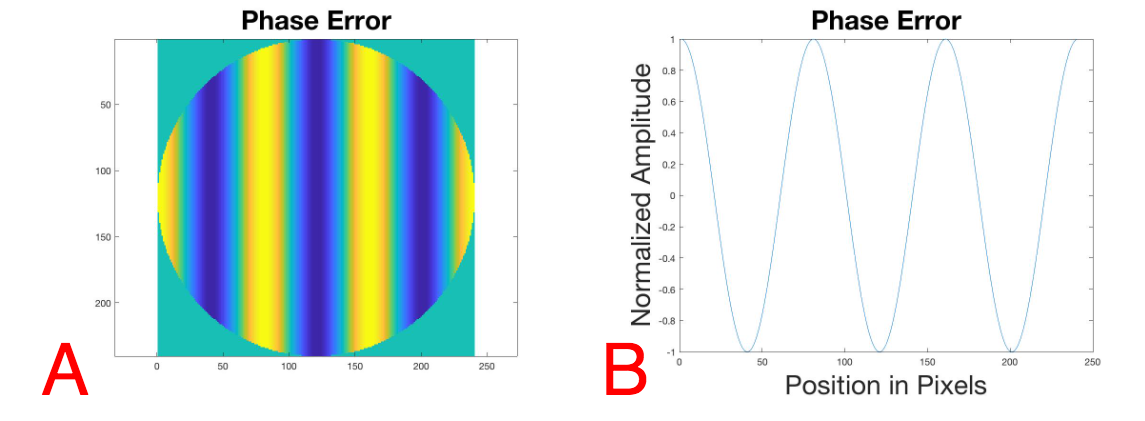
\includegraphics[width=0.8\textwidth]{Chapter Materials/Chapter Two Materials/CosinePhaseDiagram.png}
    \caption{A. Applied cosine phase error in radians in pupil plane to be propagated through the PWFS. B. Scaled cross section of the phase error.}
    \label{fig:CosinePhaseDiagram}
\end{figure}

\begin{figure}
    \centering
    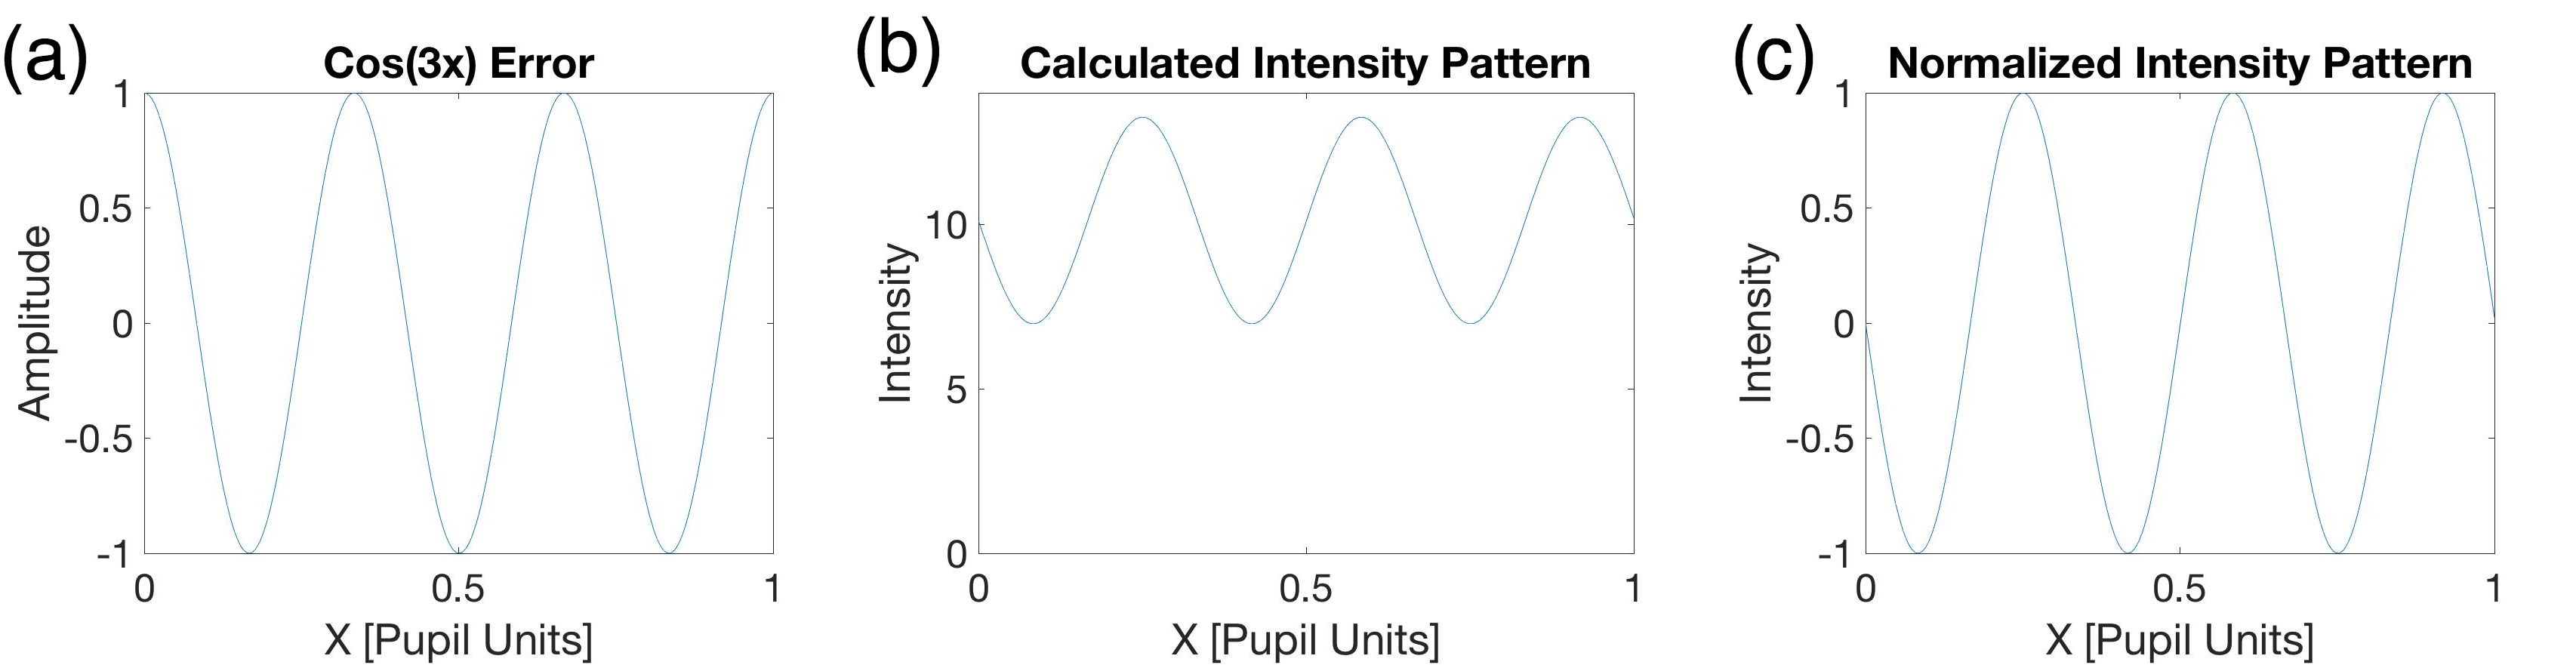
\includegraphics[width=1\textwidth]{Chapter Materials/Chapter Two Materials/MathPredictions.png}
    \caption{Predictions from the Foucault derivation. A. The applied $\cos(3x)$ phase error. B. The intensity pattern predicted for a single pupil. C. The expected pyramid signal after subtracting off constant terms and scaling.}
    \label{fig:MathPredicions}
\end{figure}

The resulting intensity patterns from the 3PWFS and 4PWFS are shown in Figure \ref{fig:IntensityPatternsDiagram} A and B. In Figure \ref{fig:IntensityPatternsDiagram} C and D we take a cross section from one of the pupils from each wavefront sensor and scale the signal. We then plot this against the predicted scaled intensity pattern. We find that the mathematical prediction is a good match for the measured intensity pattern inside the pupil of a modulated pyramid when the signal is linear. 


\begin{figure}
    \centering
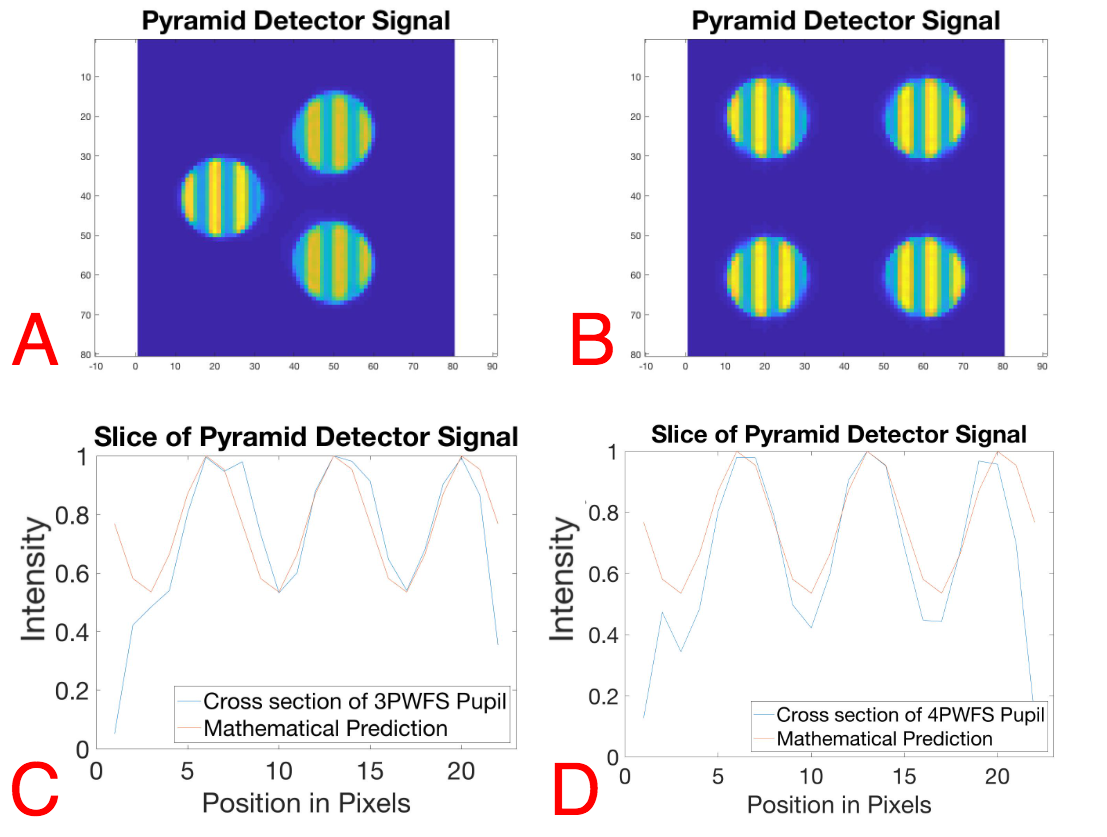
\includegraphics[width=0.8\textwidth]{Chapter Materials/Chapter Two Materials/IntensityPatternsDiagram.png}
    \caption{Resulting intensity patterns on the PWFS detector from A. the 3PWFS, and B. the 4PWFS. Figures C. and D. are cross section of the intensity pattern plotted against the mathematical prediction. For C. The cross section was taken from center of the middle-left pupil. For D. The cross section was taken from the center of the top two pupils.}
    \label{fig:IntensityPatternsDiagram}
\end{figure}

To gain further clarity we use the Slopes Maps equation that subtracts off the constant intensity and turns the signal into a pure X and Y measurement of phase. The Slopes Maps naturally subtracts the flat wavefront response and in that way is self-referencing.  More details on the Slopes calculation  for the 3PWFS is in Section~\ref{Slopes}. The Slopes Maps for the 3PWFS and the 4PWFS are shown in Figure \ref{fig:SlopesMapDiagram}, as well as the cross sections that are indeed a $-\sin(nx)$ function. 

\begin{figure}
    \centering
    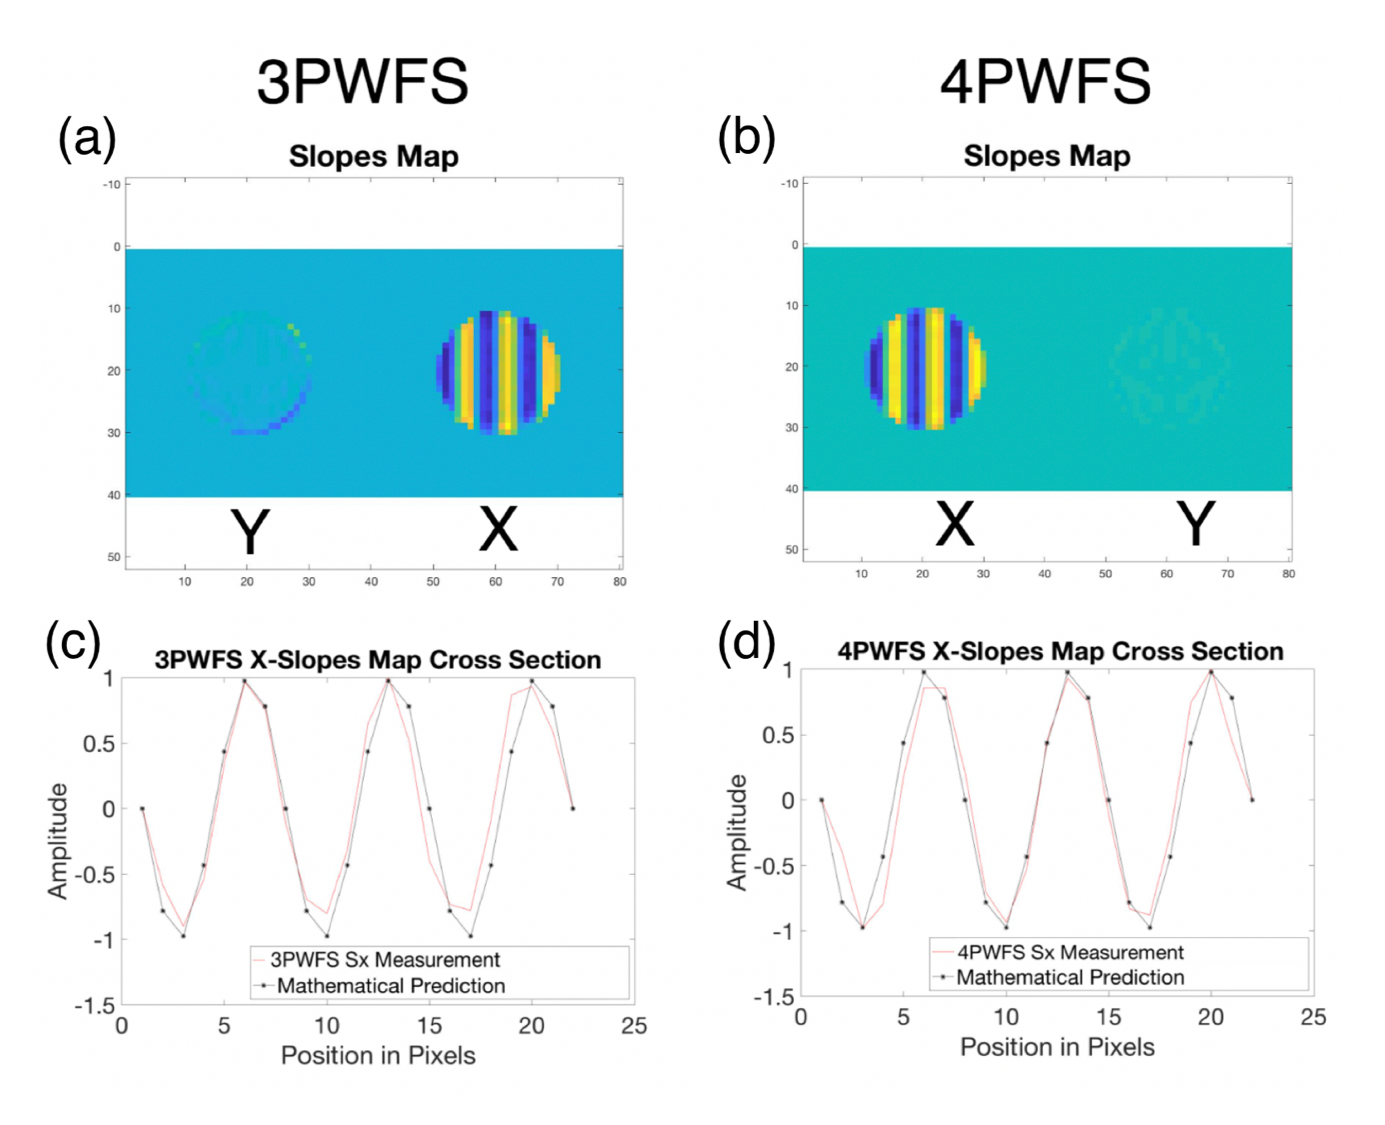
\includegraphics[width=0.9\textwidth]{Chapter Materials/Chapter Two Materials/SlopesandSlices.png}
    \caption{A. and B. Calculated slopes from the pyramid pupils. C. and D. Cross section of the Slopes plotted against the predicted signal. }
    \label{fig:SlopesMapDiagram}
\end{figure}

The previous simulations were performed with $5\lambda/D$ modulation. We can consider the 0 modulation case, which is a more direct relation to the results from the derivation. The unmodulated PWFS signal is more nonlinear than the modulated pyramid and therefore the fit between the prediction and the measured signal will be poor. In the case of the Slopes Maps signal, we found in simulation that the self-referencing is degraded from a nonlinear signal, and to return to a closer estimate of the signal the flat wavefront reference signal should be subtracted off. The fit worsens for the Slopes Maps without reference subtraction when there is a misregistration of the pupils, as will always be the case for the 3PWFS. For the 3PWFS subtracting off a reference improved the mean square error of the fit of simulation to derivation by about a factor of two, from 0.216 without subtraction, to 0.098 in the reference subtracted case. Figure \ref{fig:Mod0} summarizes the findings from the simulations with 0 modulation. Figure \ref{fig:Mod0}.A and \ref{fig:Mod0}.B are the detector signal of the 4PWFS and 3PWFS to the $\cos(3x)$ phase error. Figure \ref{fig:Mod0}.C and \ref{fig:Mod0}.D are a cross section of the scaled Slopes Maps plotted against the predicted signal. Figure \ref{fig:Mod0}.E and Figure \ref{fig:Mod0}. F are cross sections of the Slopes Maps with the reference signal subtracted.

\begin{figure}
    \centering
    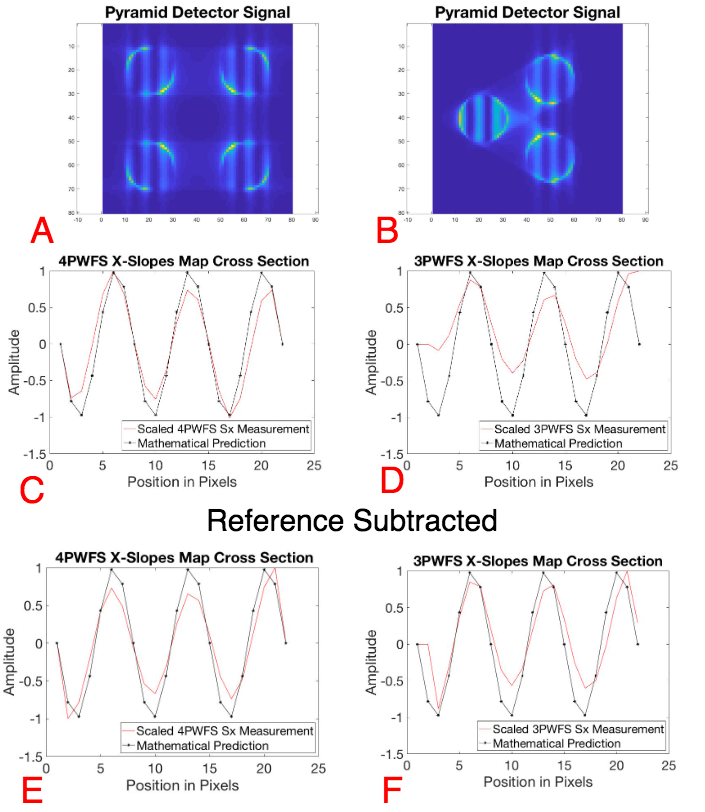
\includegraphics[width=0.9\textwidth]{Chapter Materials/Chapter Two Materials/Mod0PredictionVsSIm.png}
    \caption{A. and B. The wavefront sensor detector signals. C. and D. cross section of the wavefront sensor Slopes Maps plotted against the prediction. E. and F. the cross section of the Slopes Maps with the reference signal subtracted.}
    \label{fig:Mod0}
\end{figure}

The diffraction theory of the Foucault test predicts an intensity pattern that is the Hilbert transform of the wavefront phase. The result is an intensity pattern that is related to the wavefront derivative, but is not quite the derivative. In the case of a derivative wavefront sensor such as the Shack-Hartmann, the operation of the wavefront sensor on the phase to signal measurement is $\frac{d}{dx}\cos(nx)=-n\sin(nx)$. In the case of the pyramid the reference subtracted result is  $\frac{d}{dx}\cos(nx)=-\sin(nx)$, which is similar to the derivative wavefront sensor but without the scaling by spatial frequency. The result is that the knife edge and therefore the unmodulated pyramid sensitivity does not depend on spatial frequency as found in previous work by \cite{guyon2005}, because all spatial frequencies will produce an equally strong signal. In the Shack-Hartmann case the strength of the signal scales linearly with spatial frequency.


\section{3PWFS Slopes Maps}\label{Slopes}

\subsection{Derivation}\label{SlopesDerivation}

The Slopes Maps technique was derived for the 4PWFS using the same intensity centroid calculation as a Shack-Hartmann wavefront sensor. The Shack-Hartmann uses a quad-cell intensity calculation to track the movement of spots to calculate the X and Y gradient of the wavefront phase in post-processing. In the geometric optics approximation the PWFS acts as a slope sensor, and the Slopes Maps calculates the wavefront gradients in a similar way to the Shack-Hartmann. In the diffractive optics derivation, the wavefront slopes are calculated by the diffraction of the pyramid edges and encoded directly into the intensity pattern. We do not need to perform a Slopes Maps calculation for the pyramid signal because we are directly measuring a function that is related to the gradient phase error, but it is still beneficial to do so. The Slopes Maps is the natural recombination of the pyramid signals that subtracts off the constant Intensity pattern, so a reference image is not required. In a closed loop system the wavefront signal is driven towards  zero slope which arises when the PSF is centered on the pyramid tip with no phase errors. The Slopes Maps technique suffers from misalignments of the pyramid pupils; any misregistration in the sampling of the pupils with respect to each other results in a loss of performance. 

The Slopes Maps for the 4PWFS is already known. In previous work by Costa, a Slopes Map calculation for the 3PWFS was derived assuming a geometric optics approximation of the PWFS as a derivative wavefront sensor in the modulation regime \citep{buchler2004development}. In this paper we introduce a new Slope Maps method to handling the 3PWFS signals, which is derived using the intensity centroid of an equilateral triangle.

To calculate the Slopes Maps equations for the 3PWFS, we start from the same assumptions used for the 4PWFS. We assume that the maximum sensitivity of the sensor occurs when the PSF is centered at the tip of the four pyramid edges. We seek a Slopes Maps equation that drives the wavefront to zero slope, resulting in uniform intensity in the re-imaged pupils. To derive the centroid equation for the 3PWFS we start with an equilateral triangle, shown in Figure \ref{fig:triCentFig}. The center of the triangle is at the origin of a Cartesian coordinate system, and the vertices of the triangle are all an equal distance from the origin. The blue circles represent the layout of the pupils on the PWFS detector, and $I_1$ corresponds to $(x_1, y_1)$, etc. Solving for the coordinates $(x_1,y_1),(x_2,y_2), (x_3,y_3)$ gives the weights in the $S_x$ and $S_y$ Slopes Maps. 

% We can see in Equation~\ref{4PWFSslopes} that when the pixel values are equal the value of the Slopes are zero.

\begin{figure}
\begin{center}
\begin{tabular}{c}
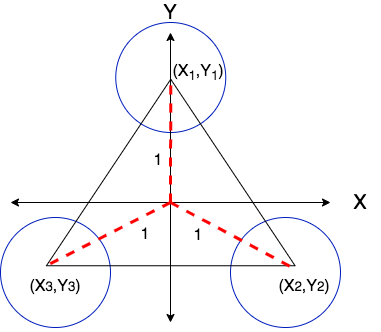
\includegraphics[height=5.5cm]{Chapter Materials/Chapter Two Materials/3PWFSslopesMap.png}
\end{tabular}
\end{center}
\caption 
{ \label{fig:triCentFig}
Equilateral triangle with the center at the origin. Solving for the coordinates of the vertex points gives the weights for the pixel Intensities used in the Slopes Maps calculation. The blue circles represent the layout of the pupils on the detector. } 
\end{figure} 

For the 3PWFS we find that the $S_x$ and $S_y$ Slopes Maps are,
% \begin{equation}
%     S_x=\frac{\frac{\sqrt{3}}{2}I_2-\frac{\sqrt{3}}{2}I_3}{I_1+I_2+I_3}, \; \;
%     S_y=\frac{I_1-\frac{1}{2}I_2-\frac{1}{2}I_3}{I_1+I_2+I_3}
%     \label{3PWFSslopes}
% \end{equation}

\begin{eqnarray}
    S_x=\frac{\frac{\sqrt{3}}{2}I_2-\frac{\sqrt{3}}{2}I_3}{I_1+I_2+I_3} \label{3PWFSslopes} \\
    S_y=\frac{I_1-\frac{1}{2}I_2-\frac{1}{2}I_3}{I_1+I_2+I_3} \nonumber
\end{eqnarray}

The $S_x$ slopes maps in this orientation depends only on the intensities from the $I_2$ and $I_3$ pupil pixels which act as a roof sensor. The result is that care must be taken to properly index the pupils when applying the Slopes Map equation. 
 
\subsection{Testbed Verification}
 
To test the validity of the Slopes Maps equation for the 3PWFS, and the Raw Intensity method we implemented these signal processing methods into a real closed adaptive optics system using the LOOPS testbed at the Laboratoire d'Astrophysique de Marseille. The LOOPS testbed at LAM used a spatial light modulator (SLM) to create the pyramid tip. A full description of the LOOPS testbed can be found in  \cite{janin2019adaptive}. On the testbed a closed loop correction was achieved for both a 3PWFS and 4PWFS with reconstructors calculated from both the Raw Intensity and Slopes Maps signal handling techniques. A reflective phase plate was used in the system to simulate turbulence, and an ALPAO deformable mirror was used to apply the correction. In all cases a stable closed loop was obtained. Figure \ref{fig:LOOOPS} shows example images from the LOOPS test-bed of (A) the pyramid signal of the 3PWFS under turbulence in closed loop, (B) the pyramid signal of the 4PWFS under turbulence in closed loop, (C) the LOOPS PSF with no turbulence, and (D) the LOOPS PSF in closed loop with the 3PWFS using the Slopes Map technique. 

\begin{figure}
    \centering
    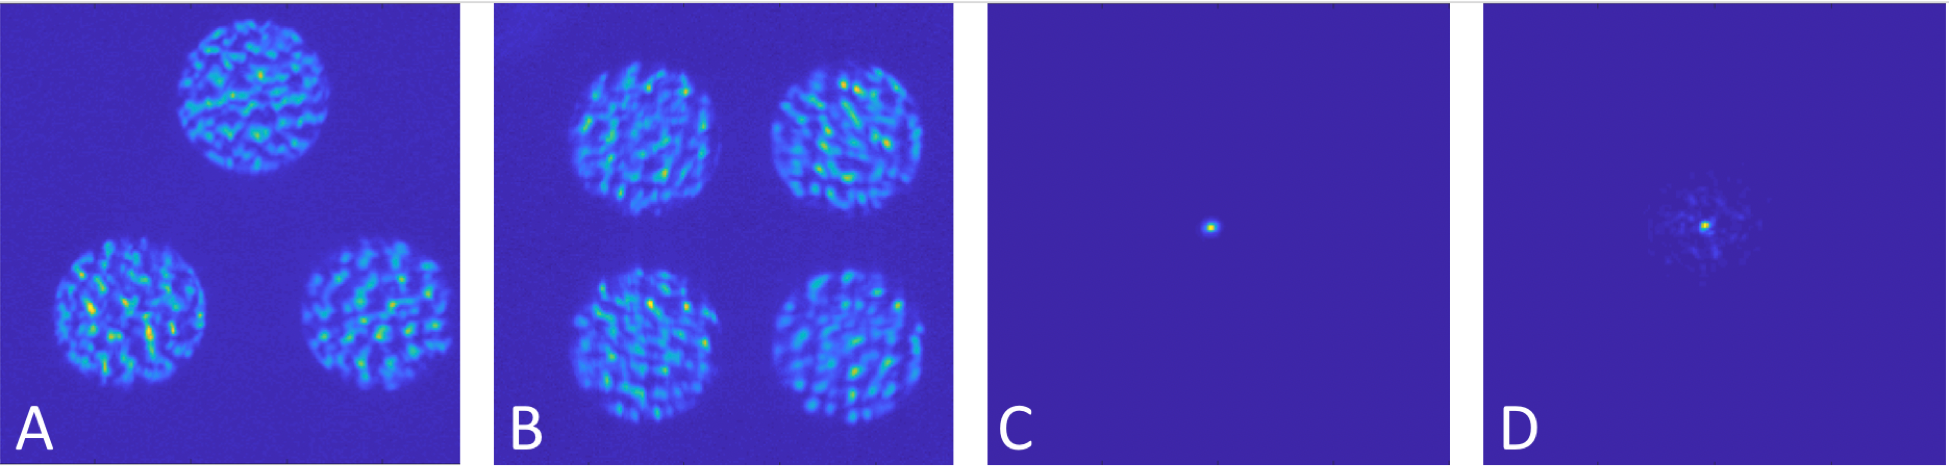
\includegraphics[width=0.8\textwidth]{Chapter Materials/Chapter Two Materials/LOOPS.png}
    \caption{Example images from the LOOPS test-bed of A) the pyramid signal of the 3PWFS under turbulence in closed loop, B) the pyramid signal of the 4PWFS under turbulence in closed loop, C) the LOOPS PSF with no turbulence, and D) the LOOPS PSF in closed loop with the 3PWFS using the Slopes Map technique.}
    \label{fig:LOOOPS}
\end{figure}

\section{The Reconstructor Matrix}

In the previous sections, we have derived what the expected signal is from the pyramid wavefront sensor, and how to process the signal to retain only the intensity pattern due to phase errors. We will now detail the processes of building a reconstructor matrix from wavefront sensor signals that allow us to reconstruct the wavefront error.
 
The wavefront sensor measures a signal $S$, which includes the signal processing discussed in Section \ref{PWFSintro}. The signal can be decomposed into a summation of modes from a basis set. The interaction matrix, $I$, is the bridge between the deformable mirror commands and the wavefront signals. The interaction matrix is calibrated by applying modes on the deformable mirror and recording the response from the wavefront sensor. The intensity measurements are unraveled from a 2D detector image into a 1D vector and stored as a column vector in the interaction matrix. We can use the interaction matrix to apply shapes on the deformable mirror by summing modes that are weighted by amplitudes stored in the amplitude matrix $A$. The interaction matrix and the amplitude matrix are related to the wavefront sensor signal by $S=IA$. In the AO case, we measure $S$, which is a $[M\times 1]$ matrix of wavefront sensor signals from aberrated starlight, and calibrate to find $I$ which is a $[M\times N]$ matrix. The dimension $M$ is the sampling of the wavefront measurement. For the Raw Intensity method $M$ is equal to the number of pixels in the pupils, and for Slopes Maps $M$ is equal to the sampling of both the $S_x$ and $S_y$ measurement. The dimension $N$ is the number of modes in the basis set used for wavefront reconstruction. To reconstruct the signal we need to find $A$, a $[N\times 1]$ matrix the corresponding amplitudes that will give us the right wavefront shape. We cannot compute the operation $A=I^{-1}S$, because $I$ is an $[M\times N]$ size matrix and not invertible. To find $A$, a pseudo-inverse of $I$ is calculated using singular value decomposition (SVD). The SVD of I is calculated by,

\begin{equation}
    SVD(I)=U\Sigma V^T
\end{equation}

\noindent where $U$ is a $[M\times M]$ matrix, $Sigma$ is an $[M\times N]$ matrix with singular values on the diagonal, and $V$ is a $[N\times N]$ matrix. We calculate the reconstructor matrix $R$ which is the pseudo-inverse of $I$ using $U$,$V$,and $\Sigma$.

\begin{equation}
   R=V\Sigma^{\dag}U^T
\end{equation}

The Reconstructor matrix R is a $[N\times M]$ sized matrix, and we calculate the vector of modal amplitudes using:

\begin{equation}
    A=RS
    \label{ReconEq}
\end{equation}

An additional matrix $C$ of size $[K\times N]$ giving the commands to drive the deformable mirror to shapes that are modes in the basis set is needed. The amplitude matrix $A$ scales this command matrix so that the proper amplitude of each mode is applied. The multiplication $V=CA$, where $V$ is a matrix of actuator positions gives a $[K\times 1]$ vector of the deformable mirror commands where $K$ is the total number of actuators used on the deformable mirror for wavefront control.  Reshaping the $[K\times 1]$ matrix into a $[\sqrt{K}\times \sqrt{K}]$ matrix gives the command for each actuator in the deformable mirror, where the deformable mirror is a square of $\sqrt{K}\times \sqrt{K}$ actuators.